\begin{frame}{dynamic linking (very briefly)}
    \begin{itemize}
        \item \textit{dynamic linking} --- done \myemph{when application is loaded}
            \begin{itemize}
                \item idea: don't have $N$ copies of {\tt printf} on disk
                \item other type of linking: \textit{static} ({\tt gcc -static})
            \end{itemize}
        \item load executable file + its libraries into memory when app starts
        \item often extra indirection:
            \begin{itemize}
            \item {\tt call functionTable[number\_for\_printf]}
            \item linker fills in {\tt functionTable} instead of changing {\tt call}s
            \end{itemize}
    \end{itemize}
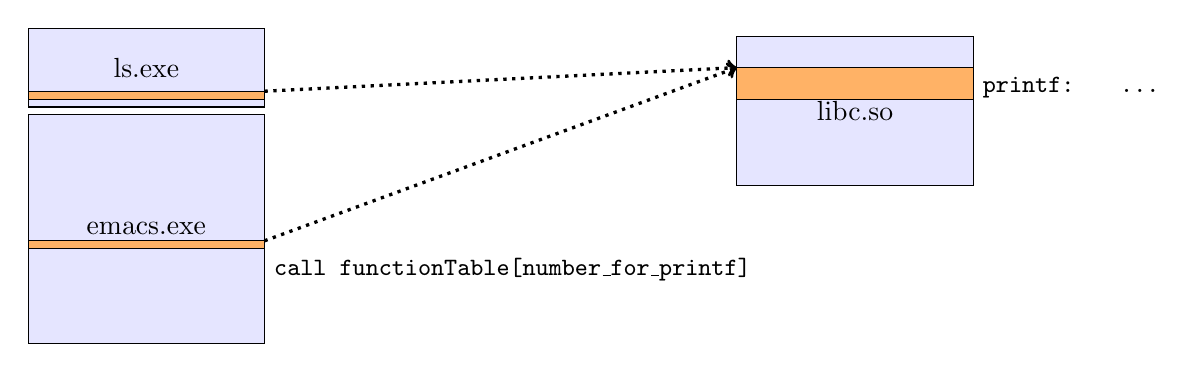
\begin{tikzpicture}
    \draw[fill=blue!10] (0, 0) rectangle (3, -1) node[midway] {ls.exe};
    \draw[fill=blue!10] (0, -1.1) rectangle (3, -4) node[midway] {emacs.exe};
    \draw[fill=blue!10] (9, -0.1) rectangle (12, -2) node[midway] {libc.so};
    \draw[fill=orange!60] (0, -.8) rectangle (3, -.9);
    \draw[fill=orange!60] (0, -2.7) rectangle (3, -2.8);
    \draw[fill=orange!60] (9, -0.5) rectangle (12, -0.9);
    \draw[very thick,->,dotted] (3, -.8) -- (9, -0.5);
    \draw[very thick,->,dotted] (3, -2.7) -- (9, -0.5);
    \node[anchor=north west,font=\fontsize{9}{10}\tt\selectfont] at (3, -2.8) {
        call functionTable[number\_for\_printf]
    };
    \node[anchor=north west,font=\fontsize{9}{10}\tt\selectfont] at (12, -0.5) {
        printf: \\
        \hspace{.25cm} \ldots
    };
\end{tikzpicture}
\end{frame}

\begin{frame}[fragile,label=lddBinLs]{\tt ldd /bin/ls}
\begin{Verbatim}[fontsize=\fontsize{12}{13}\selectfont]
$ ldd /bin/ls
    linux-vdso.so.1 =>  (0x00007ffcca9d8000)
    libselinux.so.1 => /lib/x86_64-linux-gnu/libselinux.so.1
            (0x00007f851756f000)
    libc.so.6 => /lib/x86_64-linux-gnu/libc.so.6
            (0x00007f85171a5000)
    libpcre.so.3 => /lib/x86_64-linux-gnu/libpcre.so.3
            (0x00007f8516f35000)
    libdl.so.2 => /lib/x86_64-linux-gnu/libdl.so.2
            (0x00007f8516d31000)
    /lib64/ld-linux-x86-64.so.2 (0x00007f8517791000)
    libpthread.so.0 => /lib/x86_64-linux-gnu/libpthread.so.0
            (0x00007f8516b14000)
\end{Verbatim}
\end{frame}

